\documentclass[tikz]{standalone}
\usepackage{geometry}
\usepackage{booktabs}
\geometry{a4paper,left=1.5cm,right=1.5cm, top=2cm, bottom=2cm}
\usepackage{hyperref}
\usepackage{tikz}
\usetikzlibrary{fit}
\usetikzlibrary{shapes}
\usetikzlibrary{backgrounds}
\usetikzlibrary{arrows}
\usetikzlibrary{decorations}
\usetikzlibrary{topaths}
\usetikzlibrary{patterns}
\usetikzlibrary{calc}
\usetikzlibrary{intersections}
\usetikzlibrary{through}
\usetikzlibrary{spy}
\usetikzlibrary{matrix}
\usetikzlibrary{lindenmayersystems}
\usetikzlibrary{external}
\usetikzlibrary{snakes}
\usetikzlibrary{3d}
\usepackage{anysize}
\usepackage{rotating}
\begin{document}
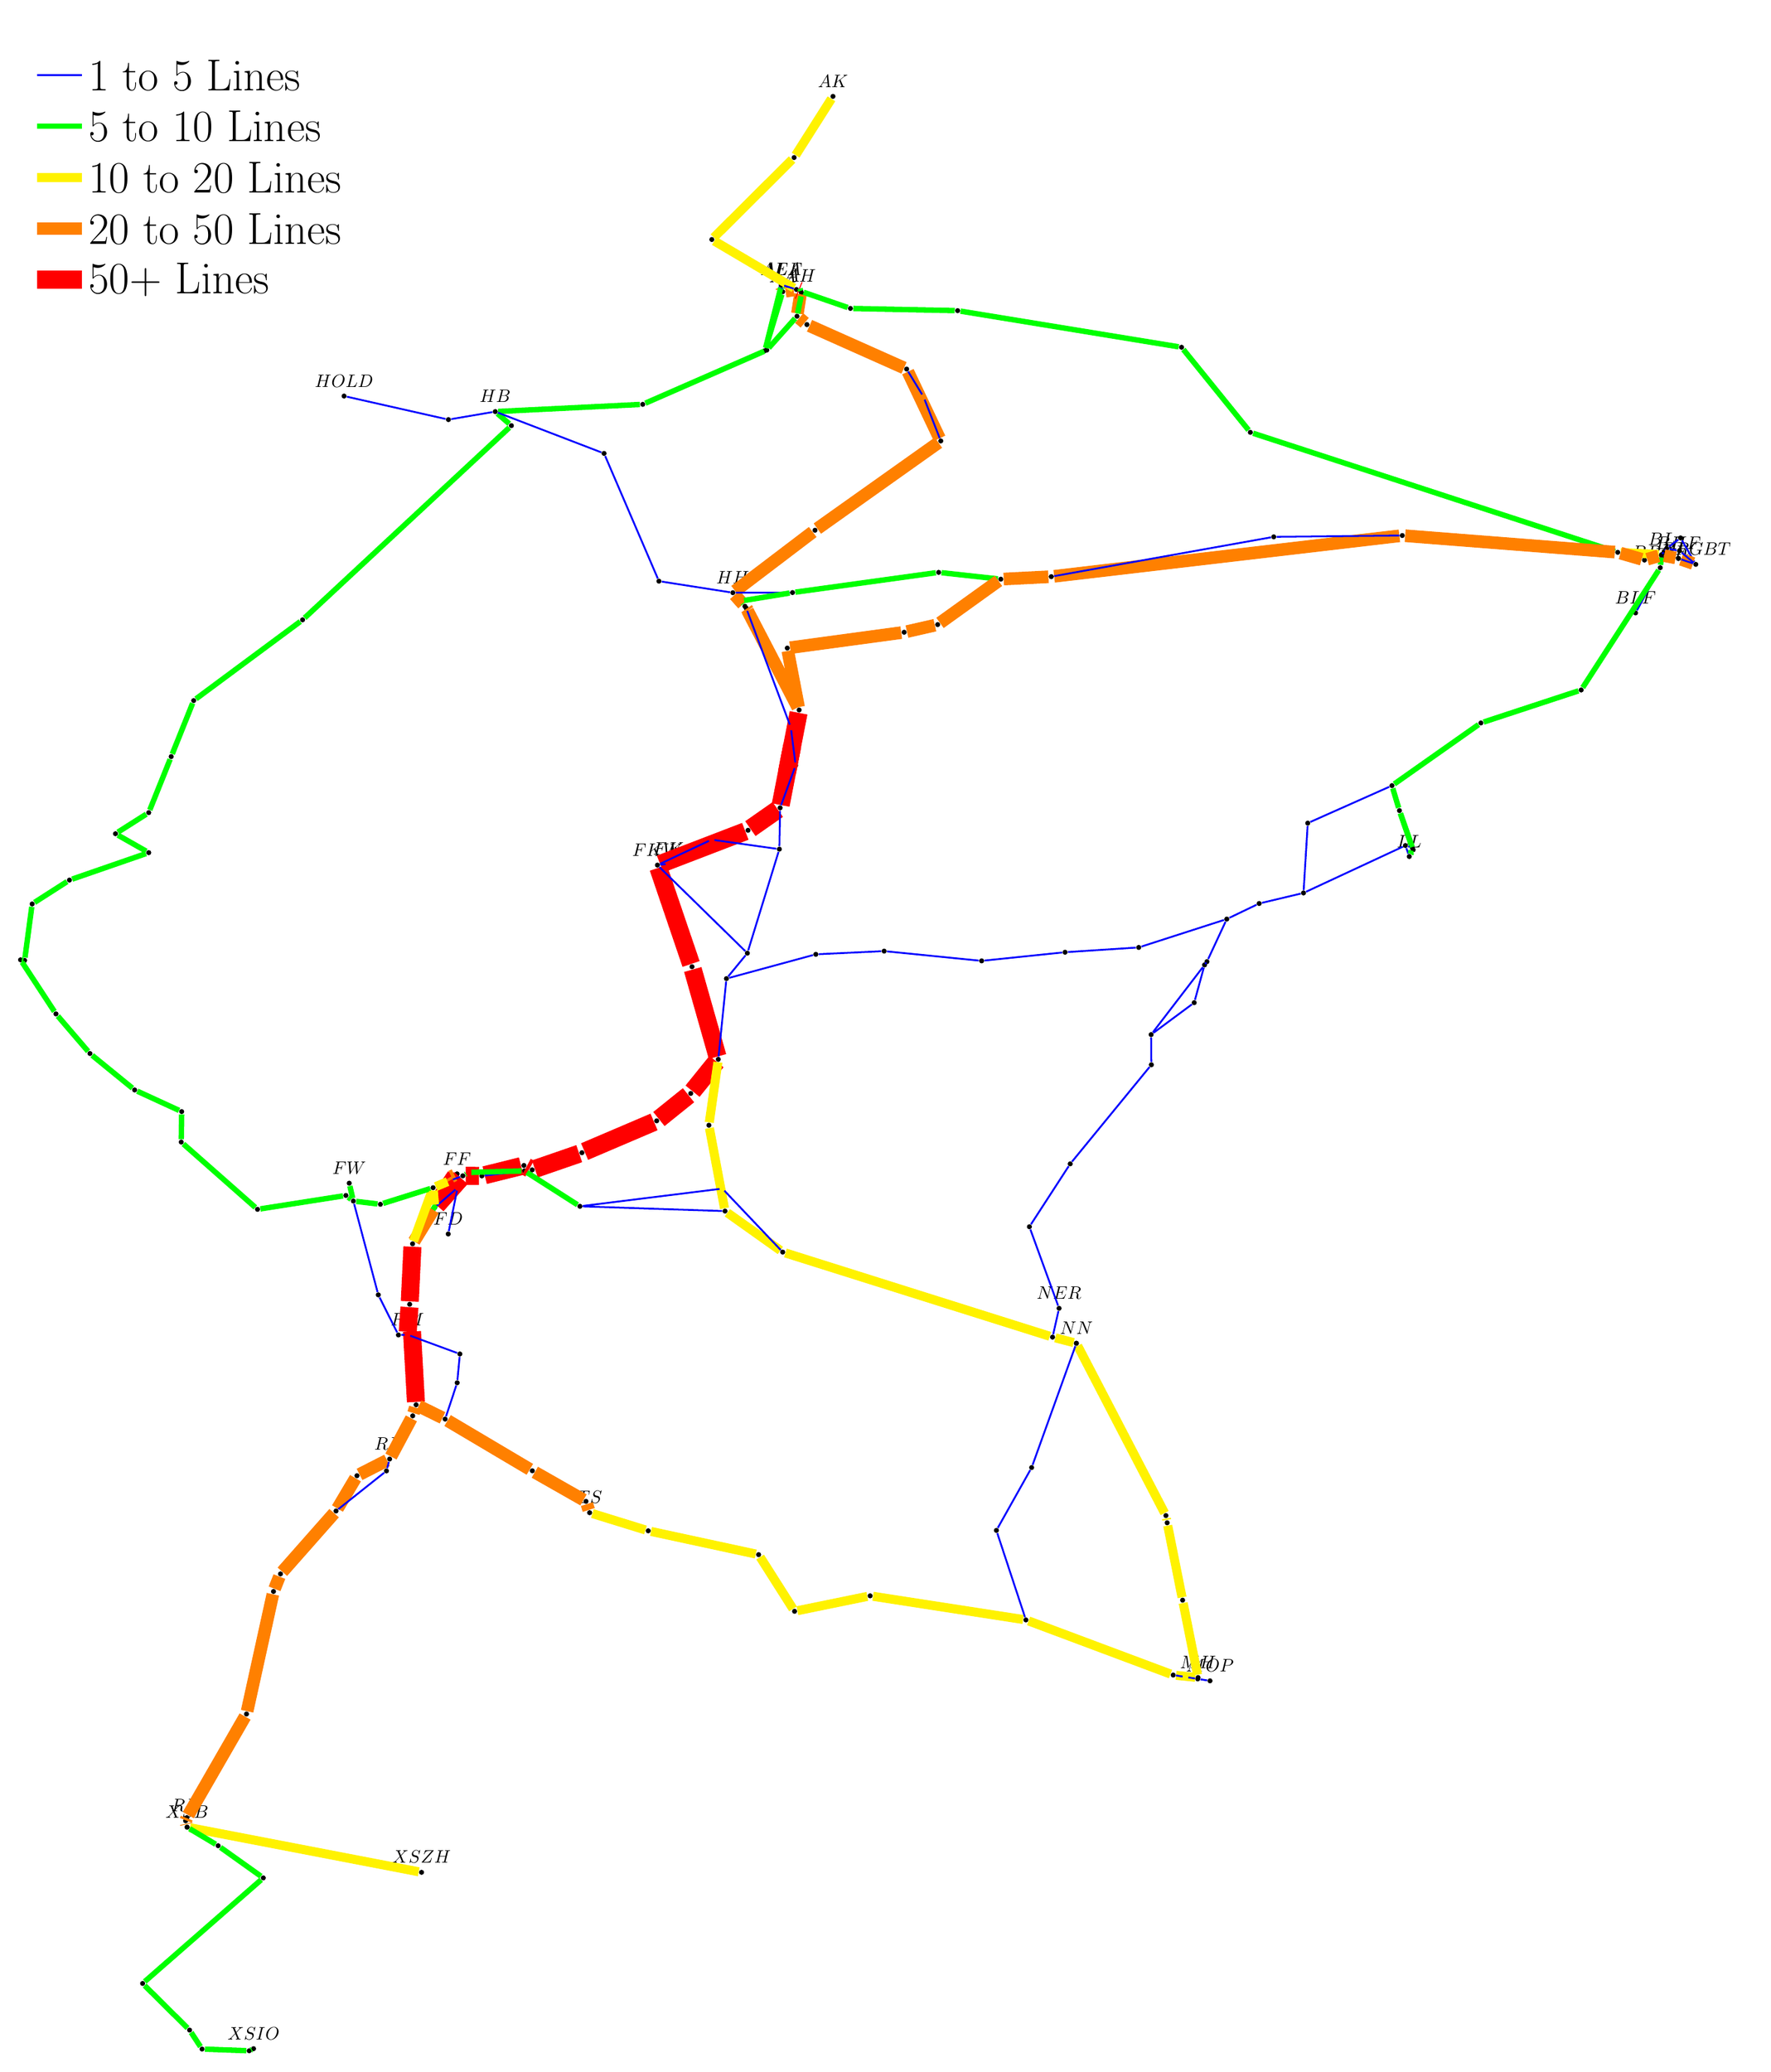
\begin{tikzpicture}[font=\normalsize]
\tikzstyle{singleLine}=[line width=1pt, blue]
\tikzstyle{fiveLines}=[line width=3pt, green]
\tikzstyle{tenLines}=[line width=5pt, yellow]
\tikzstyle{twentyLines}=[line width=7pt, orange]
\tikzstyle{fiftyLines}=[line width=10pt, red]
\node (XSZH) at (42.630379500000004,236.90263850000002)[circle, fill, inner sep=1pt, label={$XSZH$} ]{};
\node (XSB) at (38.0504215,237.7842565)[circle, fill, inner sep=1pt, label={$XSB$} ]{};
\node (RXBA) at (38.0504215,237.7842565)[circle, fill, inner sep=1pt]{};
\node (RB) at (38.021511000000004,237.90875400000002)[circle, fill, inner sep=1pt, label={$RB$} ]{};
\node (RW) at (38.046207,237.97111099999998)[circle, fill, inner sep=1pt]{};
\node (RF) at (39.21103,239.99407300000001)[circle, fill, inner sep=1pt]{};
\node (RO) at (39.738023999999996,242.38727350000002)[circle, fill, inner sep=1pt]{};
\node (RAP) at (39.8745,242.73015900000001)[circle, fill, inner sep=1pt]{};
\node (RBB) at (40.959658000000005,243.9587065)[circle, fill, inner sep=1pt]{};
\node (RDRM) at (41.3684475,244.6475365)[circle, fill, inner sep=1pt]{};
\node (RK) at (42.006637,244.972822)[circle, fill, inner sep=1pt, label={$RK$} ]{};
\node (RGN) at (42.4574685,245.816676)[circle, fill, inner sep=1pt]{};
\node (RSAB) at (42.523613999999995,246.03223)[circle, fill, inner sep=1pt]{};
\node (RP) at (42.440020000000004,247.52045249999998)[circle, fill, inner sep=1pt]{};
\node (RM) at (42.356426,247.4008675)[circle, fill, inner sep=1pt, label={$RM$} ]{};
\node (FLP) at (42.39787749999999,247.995119)[circle, fill, inner sep=1pt]{};
\node (FGE) at (42.4548985,249.17565)[circle, fill, inner sep=1pt]{};
\node (FNI) at (43.190287,250.4121825)[circle, fill, inner sep=1pt]{};
\node (FF) at (43.323874,250.5415065)[circle, fill, inner sep=1pt, label={$FF$} ]{};
\node (FMST) at (42.889386,249.88587800000002)[circle, fill, inner sep=1pt]{};
\node (FFS) at (43.436479500000004,250.503676)[circle, fill, inner sep=1pt]{};
\node (FO) at (43.808456,250.50212899999997)[circle, fill, inner sep=1pt]{};
\node (FH  N) at (44.629705,250.70619)[circle, fill, inner sep=1pt]{};
\node (FWFG) at (44.790679000000004,250.619643)[circle, fill, inner sep=1pt]{};
\node (FHME) at (45.763191,250.9550395)[circle, fill, inner sep=1pt]{};
\node (FSA) at (47.2234175,251.577949)[circle, fill, inner sep=1pt]{};
\node (FFD) at (47.888715,252.112858)[circle, fill, inner sep=1pt]{};
\node (FFU) at (48.4264835,252.778661)[circle, fill, inner sep=1pt]{};
\node (FKHM) at (47.912997,254.5869745)[circle, fill, inner sep=1pt]{};
\node (FKW) at (47.2377625,256.5716165)[circle, fill, inner sep=1pt, label={$FKW$} ]{};
\node (HJD) at (49.00723,257.25138000000004)[circle, fill, inner sep=1pt]{};
\node (HG) at (49.634425,257.689653)[circle, fill, inner sep=1pt]{};
\node (HORX) at (49.882104,258.96377)[circle, fill, inner sep=1pt]{};
\node (HAL) at (49.758264499999996,258.3267115)[circle, fill, inner sep=1pt]{};
\node (HSOR) at (50.0059435,259.60082950000003)[circle, fill, inner sep=1pt]{};
\node (HHML) at (48.972885000000005,261.588143)[circle, fill, inner sep=1pt]{};
\node (HWU) at (48.947278,261.6251055)[circle, fill, inner sep=1pt]{};
\node (HH) at (48.7109495,261.8908175)[circle, fill, inner sep=1pt, label={$HH$} ]{};
\node (HC) at (50.315811000000004,263.110206)[circle, fill, inner sep=1pt]{};
\node (HU) at (52.772835,264.8542535)[circle, fill, inner sep=1pt]{};
\node (ALBG) at (52.106030499999996,266.2579105)[circle, fill, inner sep=1pt]{};
\node (AMD) at (50.1575565,267.126624)[circle, fill, inner sep=1pt]{};
\node (AHAR) at (49.964059,267.2891375)[circle, fill, inner sep=1pt]{};
\node (AH) at (50.040416,267.7759755)[circle, fill, inner sep=1pt, label={$AH$} ]{};
\node (ADF) at (49.95283,267.8118985)[circle, fill, inner sep=1pt]{};
\node (AA) at (49.684351500000005,267.768275)[circle, fill, inner sep=1pt, label={$AA$} ]{};
\node (AK) at (50.6668775,271.5828765)[circle, fill, inner sep=1pt, label={$AK$} ]{};
\node (AN) at (49.907695,270.388252)[circle, fill, inner sep=1pt]{};
\node (AEL) at (48.30028300000001,268.78778950000003)[circle, fill, inner sep=1pt]{};
\node (FGUR) at (43.160166999999994,250.464958)[circle, fill, inner sep=1pt]{};
\node (AE  F) at (49.660669000000006,267.90412)[circle, fill, inner sep=1pt, label={$AE  F$} ]{};
\node (HN) at (49.937709999999996,258.519565)[circle, fill, inner sep=1pt]{};
\node (HK) at (49.8430065,259.261637)[circle, fill, inner sep=1pt]{};
\node (FFLF) at (42.855841999999996,250.271614)[circle, fill, inner sep=1pt]{};
\node (XSLI) at (38.656745,237.42219500000002)[circle, fill, inner sep=1pt]{};
\node (XSOL) at (39.539077,236.7936315)[circle, fill, inner sep=1pt]{};
\node (XSBE) at (37.181436,234.732691)[circle, fill, inner sep=1pt]{};
\node (XSTH) at (38.0992805,233.82151700000003)[circle, fill, inner sep=1pt]{};
\node (XSSP) at (38.342556,233.45143199999998)[circle, fill, inner sep=1pt]{};
\node (XSI) at (39.2634295,233.41785600000003)[circle, fill, inner sep=1pt]{};
\node (XSIO) at (39.348749,233.458019)[circle, fill, inner sep=1pt, label={$XSIO$} ]{};
\node (HEBG) at (49.6194335,256.882622)[circle, fill, inner sep=1pt]{};
\node (FB) at (48.994472,254.85212950000002)[circle, fill, inner sep=1pt]{};
\node (FBHF) at (48.585941999999996,254.354697)[circle, fill, inner sep=1pt]{};
\node (ALA) at (49.660669000000006,267.90412)[circle, fill, inner sep=1pt, label={$ALA$} ]{};
\node (ABG) at (51.0074185,267.442143)[circle, fill, inner sep=1pt]{};
\node (ABCH) at (53.1019835,267.3987295)[circle, fill, inner sep=1pt]{};
\node (WL) at (57.476175,266.6838435)[circle, fill, inner sep=1pt]{};
\node (WW) at (58.81991,265.022387)[circle, fill, inner sep=1pt]{};
\node (BSPD) at (65.9962835,262.679381)[circle, fill, inner sep=1pt]{};
\node (BL) at (66.8549825,262.634913)[circle, fill, inner sep=1pt, label={$BL$} ]{};
\node (BPAF) at (66.8267,262.378845)[circle, fill, inner sep=1pt, label={$BPAF$} ]{};
\node (BLF) at (66.3446585,261.49639149999996)[circle, fill, inner sep=1pt, label={$BLF$} ]{};
\node (LRIK) at (61.787506,263.007825)[circle, fill, inner sep=1pt]{};
\node (LOE) at (54.931615,262.204365)[circle, fill, inner sep=1pt]{};
\node (HWOB) at (53.945617999999996,262.15482399999996)[circle, fill, inner sep=1pt]{};
\node (HGI) at (52.730931999999996,262.287918)[circle, fill, inner sep=1pt]{};
\node (HLER) at (49.876709500000004,261.89342650000003)[circle, fill, inner sep=1pt]{};
\node (BRGBT) at (67.521285,262.444085)[circle, fill, inner sep=1pt, label={$BRGBT$} ]{};
\node (BBKB) at (67.2232765,262.9606265)[circle, fill, inner sep=1pt]{};
\node (BGS) at (66.95105,262.753291)[circle, fill, inner sep=1pt]{};
\node (BWDG) at (66.9030165,262.694102)[circle, fill, inner sep=1pt]{};
\node (BJUE) at (65.282042,259.99125)[circle, fill, inner sep=1pt]{};
\node (LW) at (63.32378249999999,259.3472745)[circle, fill, inner sep=1pt]{};
\node (LBT) at (61.586023499999996,258.1233285)[circle, fill, inner sep=1pt]{};
\node (LDL) at (61.732223,257.6359765)[circle, fill, inner sep=1pt]{};
\node (LNW S) at (62.000225,256.86962)[circle, fill, inner sep=1pt]{};
\node (LL) at (61.9244105,256.7391445)[circle, fill, inner sep=1pt, label={$LL$} ]{};
\node (LWI) at (61.8488385,256.95392)[circle, fill, inner sep=1pt]{};
\node (UW) at (59.857968,256.0273535)[circle, fill, inner sep=1pt]{};
\node (UNM) at (58.9922915,255.8216285)[circle, fill, inner sep=1pt]{};
\node (USK) at (58.359127,255.5172405)[circle, fill, inner sep=1pt]{};
\node (UWM) at (56.639233000000004,254.963652)[circle, fill, inner sep=1pt]{};
\node (UE  P) at (55.200318499999995,254.87026149999997)[circle, fill, inner sep=1pt]{};
\node (UGO) at (53.570744499999996,254.70139799999998)[circle, fill, inner sep=1pt]{};
\node (UEI) at (51.666078999999996,254.89201500000001)[circle, fill, inner sep=1pt]{};
\node (UGT) at (50.331788,254.82914350000001)[circle, fill, inner sep=1pt]{};
\node (HHI) at (49.774266000000004,260.80938199999997)[circle, fill, inner sep=1pt]{};
\node (HGGL) at (52.0569575,261.118667)[circle, fill, inner sep=1pt]{};
\node (HBS) at (52.7117405,261.2682415)[circle, fill, inner sep=1pt]{};
\node (BCHB) at (66.51803100000001,262.5283905)[circle, fill, inner sep=1pt]{};
\node (BLS) at (66.8473,262.625055)[circle, fill, inner sep=1pt]{};
\node (BHF) at (67.181558,262.56030150000004)[circle, fill, inner sep=1pt, label={$BHF$} ]{};
\node (BOSGA) at (67.181558,262.56030150000004)[circle, fill, inner sep=1pt]{};
\node (FNIS) at (43.333580500000004,250.27088500000002)[circle, fill, inner sep=1pt]{};
\node (FD) at (43.1512785,249.36812799999998)[circle, fill, inner sep=1pt, label={$FD$} ]{};
\node (RROL) at (43.090416,245.75336700000003)[circle, fill, inner sep=1pt]{};
\node (TV) at (44.7939255,244.74373350000002)[circle, fill, inner sep=1pt]{};
\node (TSZ) at (45.842501999999996,244.1471165)[circle, fill, inner sep=1pt]{};
\node (TS) at (45.913448,243.92547100000002)[circle, fill, inner sep=1pt, label={$TS$} ]{};
\node (ABLZ) at (49.374916999999996,266.62874999999997)[circle, fill, inner sep=1pt]{};
\node (AROG) at (46.950962000000004,265.5689395)[circle, fill, inner sep=1pt]{};
\node (HB) at (44.0699975,265.4272305)[circle, fill, inner sep=1pt, label={$HB$} ]{};
\node (HGA) at (44.385192499999995,265.153426)[circle, fill, inner sep=1pt]{};
\node (HO  O) at (40.30619,261.360955)[circle, fill, inner sep=1pt]{};
\node (EMSTP) at (38.179475,259.78446)[circle, fill, inner sep=1pt]{};
\node (EMSTG) at (37.74001175,258.6902685)[circle, fill, inner sep=1pt]{};
\node (EDO) at (37.300548500000005,257.596077)[circle, fill, inner sep=1pt]{};
\node (EWIT) at (36.6512595,257.1842965)[circle, fill, inner sep=1pt]{};
\node (EHG) at (37.3008935,256.814601)[circle, fill, inner sep=1pt]{};
\node (KW) at (35.752272,256.27887699999997)[circle, fill, inner sep=1pt]{};
\node (KSO) at (35.0238445,255.812763)[circle, fill, inner sep=1pt]{};
\node (KKDZ) at (34.876478500000005,254.71067449999998)[circle, fill, inner sep=1pt]{};
\node (KK) at (34.7973445,254.721426)[circle, fill, inner sep=1pt]{};
\node (KB) at (35.489004,253.6658735)[circle, fill, inner sep=1pt]{};
\node (KRE) at (36.152863499999995,252.892142)[circle, fill, inner sep=1pt]{};
\node (KAND) at (37.026028000000004,252.180585)[circle, fill, inner sep=1pt]{};
\node (KKO) at (37.9446135,251.75826849999999)[circle, fill, inner sep=1pt]{};
\node (KBOP) at (37.935724,251.163119)[circle, fill, inner sep=1pt]{};
\node (FBGK) at (39.4257465,249.84936900000002)[circle, fill, inner sep=1pt]{};
\node (FMM) at (41.15276299999999,250.1200175)[circle, fill, inner sep=1pt]{};
\node (FMZ) at (41.29831850000001,250.01130899999998)[circle, fill, inner sep=1pt]{};
\node (FMB P) at (41.82626,249.94834999999998)[circle, fill, inner sep=1pt]{};
\node (NMOT) at (48.2434075,251.49170949999998)[circle, fill, inner sep=1pt]{};
\node (NRB) at (48.558071,249.8149015)[circle, fill, inner sep=1pt]{};
\node (NWH) at (49.68477,249.0145645)[circle, fill, inner sep=1pt]{};
\node (NF) at (54.95607,247.353879)[circle, fill, inner sep=1pt]{};
\node (NN) at (55.4215465,247.233385)[circle, fill, inner sep=1pt, label={$NN$} ]{};
\node (NRWD) at (55.4215465,247.233385)[circle, fill, inner sep=1pt]{};
\node (MIN) at (57.170768,243.8690955)[circle, fill, inner sep=1pt]{};
\node (MIH) at (57.1948545,243.7284205)[circle, fill, inner sep=1pt]{};
\node (MAKN) at (57.496703499999995,242.21710900000002)[circle, fill, inner sep=1pt]{};
\node (MH) at (57.798553000000005,240.70579800000002)[circle, fill, inner sep=1pt, label={$MH$} ]{};
\node (ABIL) at (52.43697949999999,265.7139675)[circle, fill, inner sep=1pt]{};
\node (AA  G) at (49.337625,266.616945)[circle, fill, inner sep=1pt]{};
\node (ALAA) at (49.654315000000004,267.897975)[circle, fill, inner sep=1pt]{};
\node (LLMO) at (61.98238,256.9109635)[circle, fill, inner sep=1pt]{};
\node (MP) at (57.312971,240.755001)[circle, fill, inner sep=1pt]{};
\node (MA) at (54.4355185,241.83161299999998)[circle, fill, inner sep=1pt]{};
\node (MGZB) at (51.392881499999994,242.3018605)[circle, fill, inner sep=1pt]{};
\node (TU) at (49.9166485,241.99985600000002)[circle, fill, inner sep=1pt]{};
\node (TG) at (49.214096999999995,243.10639250000003)[circle, fill, inner sep=1pt]{};
\node (TP) at (47.058010499999995,243.571678)[circle, fill, inner sep=1pt]{};
\node (AERI) at (50.055814999999996,267.73172999999997)[circle, fill, inner sep=1pt]{};
\node (RH) at (43.378949999999996,247.0251265)[circle, fill, inner sep=1pt]{};
\node (RWS) at (43.326313,246.462289)[circle, fill, inner sep=1pt]{};
\node (LH) at (59.9412655,257.3912395)[circle, fill, inner sep=1pt]{};
\node (UJS) at (57.972073,254.686344)[circle, fill, inner sep=1pt]{};
\node (UJP) at (57.925544,254.62271049999998)[circle, fill, inner sep=1pt]{};
\node (UO) at (57.723073,253.885028)[circle, fill, inner sep=1pt]{};
\node (US) at (56.881792000000004,253.261648)[circle, fill, inner sep=1pt]{};
\node (UPR) at (56.886255500000004,252.6721995)[circle, fill, inner sep=1pt]{};
\node (NLF) at (55.3011755,250.73772300000002)[circle, fill, inner sep=1pt]{};
\node (NBA) at (54.50392049999999,249.509243)[circle, fill, inner sep=1pt]{};
\node (NER) at (55.083335,247.91666500000002)[circle, fill, inner sep=1pt, label={$NER$} ]{};
\node (FHMD) at (48.2955665,257.0689015)[circle, fill, inner sep=1pt]{};
\node (RETL) at (41.944193500000004,244.740942)[circle, fill, inner sep=1pt]{};
\node (FK) at (47.4531245,256.5977625)[circle, fill, inner sep=1pt, label={$FK$} ]{};
\node (FW) at (41.217388,250.3597135)[circle, fill, inner sep=1pt, label={$FW$} ]{};
\node (NAH) at (45.7237825,249.90846449999998)[circle, fill, inner sep=1pt]{};
\node (FH  S) at (44.64011,250.60013999999998)[circle, fill, inner sep=1pt]{};
\node (FWOR) at (41.78529,248.17965099999998)[circle, fill, inner sep=1pt]{};
\node (RL) at (42.178487000000004,247.39594499999998)[circle, fill, inner sep=1pt]{};
\node (HWAM) at (48.87414,261.72965999999997)[circle, fill, inner sep=1pt]{};
\node (MOP) at (58.0317995,240.6417945)[circle, fill, inner sep=1pt, label={$MOP$} ]{};
\node (MAFB) at (57.792190000000005,240.67953)[circle, fill, inner sep=1pt]{};
\node (MLR) at (57.552580500000005,240.7172655)[circle, fill, inner sep=1pt]{};
\node (MDT) at (53.8589815,243.57953250000003)[circle, fill, inner sep=1pt]{};
\node (MTL) at (54.5477155,244.80683599999998)[circle, fill, inner sep=1pt]{};
\node (LS) at (59.277010499999996,262.981636)[circle, fill, inner sep=1pt]{};
\node (NGM) at (48.507155,250.254223)[circle, fill, inner sep=1pt]{};
\node (FFO) at (43.546727000000004,250.570042)[circle, fill, inner sep=1pt]{};
\node (BGFB) at (67.204234,262.708513)[circle, fill, inner sep=1pt]{};
\node (HWUN) at (47.2672425,262.1164175)[circle, fill, inner sep=1pt]{};
\node (HV) at (46.1952845,264.6107485)[circle, fill, inner sep=1pt]{};
\node (HD) at (43.154998000000006,265.271276)[circle, fill, inner sep=1pt]{};
\node (HOLD) at (41.117,265.73095850000004)[circle, fill, inner sep=1pt, label={$HOLD$} ]{};
\node (max) at (68.521285,272.5828765){};
\draw[tenLines] (XSZH) to (XSB);
\draw[twentyLines] (XSB) to (RXBA);
\draw[twentyLines] (RXBA) to (RB);
\draw[twentyLines] (RB) to (RW);
\draw[twentyLines] (RW) to (RF);
\draw[twentyLines] (RF) to (RO);
\draw[twentyLines] (RO) to (RAP);
\draw[twentyLines] (RAP) to (RBB);
\draw[twentyLines] (RBB) to (RDRM);
\draw[twentyLines] (RDRM) to (RK);
\draw[twentyLines] (RK) to (RGN);
\draw[twentyLines] (RGN) to (RSAB);
\draw[fiftyLines] (RSAB) to (RP);
\draw[fiftyLines] (RP) to (RM);
\draw[fiftyLines] (RM) to (FLP);
\draw[fiftyLines] (FLP) to (FGE);
\draw[fiveLines] (FGE) to (FNI);
\draw[fiveLines] (FNI) to (FF);
\draw[fiftyLines] (FF) to (FMST);
\draw[twentyLines] (FMST) to (FGE);
\draw[fiftyLines] (FMST) to (FFS);
\draw[fiftyLines] (FFS) to (FO);
\draw[fiftyLines] (FO) to (FH  N);
\draw[fiftyLines] (FH  N) to (FWFG);
\draw[fiftyLines] (FWFG) to (FHME);
\draw[fiftyLines] (FHME) to (FSA);
\draw[fiftyLines] (FSA) to (FFD);
\draw[fiftyLines] (FFD) to (FFU);
\draw[fiftyLines] (FFU) to (FKHM);
\draw[fiftyLines] (FKHM) to (FKW);
\draw[fiftyLines] (FKW) to (HJD);
\draw[fiftyLines] (HJD) to (HG);
\draw[fiftyLines] (HG) to (HORX);
\draw[fiftyLines] (HORX) to (HAL);
\draw[fiftyLines] (HAL) to (HSOR);
\draw[twentyLines] (HSOR) to (HHML);
\draw[twentyLines] (HHML) to (HWU);
\draw[twentyLines] (HWU) to (HH);
\draw[twentyLines] (HH) to (HC);
\draw[twentyLines] (HC) to (HU);
\draw[twentyLines] (HU) to (ALBG);
\draw[twentyLines] (ALBG) to (AMD);
\draw[twentyLines] (AMD) to (AHAR);
\draw[twentyLines] (AHAR) to (AH);
\draw[fiftyLines] (AH) to (ADF);
\draw[twentyLines] (ADF) to (AA);
\draw[tenLines] (AK) to (AN);
\draw[tenLines] (AN) to (AEL);
\draw[tenLines] (AEL) to (ADF);
\draw[twentyLines] (FF) to (FGUR);
\draw[twentyLines] (FGUR) to (FNI);
\draw[twentyLines] (AA) to (AE  F);
\draw[singleLine] (HG) to (HN);
\draw[singleLine] (HN) to (HK);
\draw[singleLine] (HK) to (HHML);
\draw[tenLines] (FNI) to (FFLF);
\draw[tenLines] (FFLF) to (FGE);
\draw[fiveLines] (XSB) to (XSLI);
\draw[fiveLines] (XSLI) to (XSOL);
\draw[fiveLines] (XSOL) to (XSBE);
\draw[fiveLines] (XSBE) to (XSTH);
\draw[fiveLines] (XSTH) to (XSSP);
\draw[fiveLines] (XSSP) to (XSI);
\draw[fiveLines] (XSI) to (XSIO);
\draw[singleLine] (AE  F) to (ADF);
\draw[singleLine] (HG) to (HEBG);
\draw[singleLine] (HEBG) to (FB);
\draw[singleLine] (FB) to (FBHF);
\draw[singleLine] (FBHF) to (FFU);
\draw[singleLine] (FFS) to (FNI);
\draw[fiveLines] (ALA) to (AA);
\draw[fiveLines] (AH) to (ABG);
\draw[fiveLines] (ABG) to (ABCH);
\draw[fiveLines] (ABCH) to (WL);
\draw[fiveLines] (WL) to (WW);
\draw[fiveLines] (WW) to (BSPD);
\draw[tenLines] (BSPD) to (BL);
\draw[fiveLines] (BL) to (BPAF);
\draw[singleLine] (BLF) to (BPAF);
\draw[twentyLines] (BSPD) to (LRIK);
\draw[twentyLines] (LRIK) to (LOE);
\draw[twentyLines] (LOE) to (HWOB);
\draw[fiveLines] (HWOB) to (HGI);
\draw[fiveLines] (HGI) to (HLER);
\draw[singleLine] (HLER) to (HH);
\draw[singleLine] (BRGBT) to (BBKB);
\draw[singleLine] (BBKB) to (BGS);
\draw[singleLine] (BGS) to (BWDG);
\draw[singleLine] (BWDG) to (BL);
\draw[fiveLines] (BPAF) to (BJUE);
\draw[fiveLines] (BJUE) to (LW);
\draw[fiveLines] (LW) to (LBT);
\draw[fiveLines] (LBT) to (LDL);
\draw[fiveLines] (LDL) to (LNW S);
\draw[fiveLines] (LNW S) to (LL);
\draw[singleLine] (LL) to (LWI);
\draw[singleLine] (LWI) to (UW);
\draw[singleLine] (UW) to (UNM);
\draw[singleLine] (UNM) to (USK);
\draw[singleLine] (USK) to (UWM);
\draw[singleLine] (UWM) to (UE  P);
\draw[singleLine] (UE  P) to (UGO);
\draw[singleLine] (UGO) to (UEI);
\draw[singleLine] (UEI) to (UGT);
\draw[singleLine] (UGT) to (FBHF);
\draw[twentyLines] (HSOR) to (HHI);
\draw[twentyLines] (HHI) to (HGGL);
\draw[twentyLines] (HGGL) to (HBS);
\draw[twentyLines] (HBS) to (HWOB);
\draw[twentyLines] (BSPD) to (BCHB);
\draw[twentyLines] (BCHB) to (BLS);
\draw[twentyLines] (BLS) to (BHF);
\draw[twentyLines] (BHF) to (BRGBT);
\draw[singleLine] (BHF) to (BOSGA);
\draw[singleLine] (BOSGA) to (BRGBT);
\draw[singleLine] (FMST) to (FNIS);
\draw[singleLine] (FNIS) to (FD);
\draw[twentyLines] (RSAB) to (RROL);
\draw[twentyLines] (RROL) to (TV);
\draw[twentyLines] (TV) to (TSZ);
\draw[twentyLines] (TSZ) to (TS);
\draw[fiveLines] (AHAR) to (ABLZ);
\draw[fiveLines] (ABLZ) to (AROG);
\draw[fiveLines] (AROG) to (HB);
\draw[fiveLines] (HB) to (HGA);
\draw[fiveLines] (HGA) to (HO  O);
\draw[fiveLines] (HO  O) to (EMSTP);
\draw[fiveLines] (EMSTP) to (EMSTG);
\draw[fiveLines] (EMSTG) to (EDO);
\draw[fiveLines] (EDO) to (EWIT);
\draw[fiveLines] (EWIT) to (EHG);
\draw[fiveLines] (EHG) to (KW);
\draw[fiveLines] (KW) to (KSO);
\draw[fiveLines] (KSO) to (KKDZ);
\draw[fiveLines] (KKDZ) to (KK);
\draw[fiveLines] (KK) to (KB);
\draw[fiveLines] (KB) to (KRE);
\draw[fiveLines] (KRE) to (KAND);
\draw[fiveLines] (KAND) to (KKO);
\draw[fiveLines] (KKO) to (KBOP);
\draw[fiveLines] (KBOP) to (FBGK);
\draw[fiveLines] (FBGK) to (FMM);
\draw[fiveLines] (FMM) to (FMZ);
\draw[fiveLines] (FMZ) to (FMB P);
\draw[fiveLines] (FMB P) to (FFLF);
\draw[tenLines] (FFLF) to (FMST);
\draw[tenLines] (FFU) to (NMOT);
\draw[tenLines] (NMOT) to (NRB);
\draw[tenLines] (NRB) to (NWH);
\draw[tenLines] (NWH) to (NF);
\draw[tenLines] (NF) to (NN);
\draw[tenLines] (NN) to (NRWD);
\draw[tenLines] (NRWD) to (MIN);
\draw[tenLines] (MIN) to (MIH);
\draw[tenLines] (MIH) to (MAKN);
\draw[tenLines] (MAKN) to (MH);
\draw[singleLine] (ALBG) to (ABIL);
\draw[singleLine] (ABIL) to (HU);
\draw[fiveLines] (AE  F) to (AA  G);
\draw[fiveLines] (AA  G) to (AA);
\draw[singleLine] (AA) to (ALAA);
\draw[singleLine] (ALAA) to (AE  F);
\draw[fiveLines] (LDL) to (LLMO);
\draw[fiveLines] (LLMO) to (LL);
\draw[tenLines] (MH) to (MP);
\draw[tenLines] (MP) to (MA);
\draw[tenLines] (MA) to (MGZB);
\draw[tenLines] (MGZB) to (TU);
\draw[tenLines] (TU) to (TG);
\draw[tenLines] (TG) to (TP);
\draw[tenLines] (TP) to (TS);
\draw[fiveLines] (AH) to (AERI);
\draw[fiveLines] (AERI) to (AHAR);
\draw[singleLine] (RM) to (RH);
\draw[singleLine] (RH) to (RWS);
\draw[singleLine] (RWS) to (RROL);
\draw[singleLine] (LBT) to (LH);
\draw[singleLine] (LH) to (UW);
\draw[singleLine] (USK) to (UJS);
\draw[singleLine] (UJS) to (UJP);
\draw[singleLine] (UJP) to (UO);
\draw[singleLine] (UO) to (US);
\draw[singleLine] (US) to (UPR);
\draw[singleLine] (UPR) to (NLF);
\draw[singleLine] (NLF) to (NBA);
\draw[singleLine] (NBA) to (NER);
\draw[singleLine] (NER) to (NF);
\draw[singleLine] (FKW) to (FHMD);
\draw[singleLine] (FHMD) to (HEBG);
\draw[singleLine] (RBB) to (RETL);
\draw[singleLine] (RETL) to (RK);
\draw[singleLine] (FKW) to (FK);
\draw[fiveLines] (FMZ) to (FW);
\draw[singleLine] (NRB) to (NAH);
\draw[fiveLines] (NAH) to (FH  S);
\draw[singleLine] (FH  S) to (FO);
\draw[singleLine] (FB) to (FKW);
\draw[singleLine] (FMZ) to (FWOR);
\draw[singleLine] (FWOR) to (RL);
\draw[singleLine] (RL) to (RM);
\draw[fiveLines] (HLER) to (HWAM);
\draw[fiveLines] (HWAM) to (HWU);
\draw[singleLine] (MOP) to (MAFB);
\draw[singleLine] (MAFB) to (MLR);
\draw[singleLine] (MLR) to (MP);
\draw[singleLine] (MA) to (MDT);
\draw[singleLine] (MDT) to (MTL);
\draw[singleLine] (MTL) to (NN);
\draw[singleLine] (US) to (UJP);
\draw[singleLine] (LWI) to (LLMO);
\draw[singleLine] (LOE) to (LS);
\draw[singleLine] (LS) to (LRIK);
\draw[singleLine] (NAH) to (NGM);
\draw[singleLine] (NGM) to (NWH);
\draw[fiveLines] (FH  S) to (FFO);
\draw[fiveLines] (FFO) to (FFS);
\draw[singleLine] (BGS) to (BGFB);
\draw[singleLine] (BGFB) to (BRGBT);
\draw[singleLine] (HH) to (HWUN);
\draw[singleLine] (HWUN) to (HV);
\draw[singleLine] (HV) to (HB);
\draw[singleLine] (HB) to (HD);
\draw[singleLine] (HD) to (HOLD);
\node (Dummy) at (35.0,273.0){};
\node (1LegendS) at (35.0,272.0){};
\node[anchor = west] (1LegendT) at (36.0,272.0){\Huge  1 to 5 Lines};
\draw[singleLine] (1LegendS) to (1LegendT);
\node (5LegendS) at (35.0,271.0){};
\node[anchor = west] (5LegendT) at (36.0,271.0){\Huge  5 to 10 Lines};
\draw[fiveLines] (5LegendS) to (5LegendT);
\node (10LegendS) at (35.0,270.0){};
\node[anchor = west] (10LegendT) at (36.0,270.0){\Huge 10 to 20 Lines};
\draw[tenLines] (10LegendS) to (10LegendT);
\node (20LegendS) at (35.0,269.0){};
\node[anchor = west] (20LegendT) at (36.0,269.0){\Huge 20 to 50 Lines};
\draw[twentyLines] (20LegendS) to (20LegendT);
\node (50LegendS) at (35.0,268.0){};
\node[anchor = west] (50LegendT) at (36.0,268.0){\Huge 50+      Lines};
\draw[fiftyLines] (50LegendS) to (50LegendT);
\end{tikzpicture}
\end{document}
